\documentclass[border=4pt]{standalone}
% Shared by the independently buildable vector figures.
\usepackage[T1]{fontenc}
\usepackage{amsmath,amssymb,newpxtext,newpxmath}
\usepackage[semibold]{sourcesans}
\usepackage{pgfplots}
\pgfplotsset{compat=1.18}
\usetikzlibrary{arrows.meta,calc,positioning}
\usepgfplotslibrary{groupplots}
\definecolor{ink}{HTML}{19303A}
\definecolor{sea}{HTML}{00675E}
\definecolor{clay}{HTML}{A24725}
\definecolor{muted}{HTML}{4C636C}
\definecolor{rulegray}{HTML}{CAD4D4}
\definecolor{wash}{HTML}{EAF4F0}
\definecolor{warm}{HTML}{F7EEE5}
\color{ink}
\tikzset{every picture/.style={font=\sffamily\small},
  arrow/.style={-{Stealth[length=2mm]},line width=.8pt,draw=muted}}
\pgfplotsset{companion/.style={axis lines=left,axis line style={draw=muted},
  tick style={draw=muted},ticklabel style={font=\sffamily\footnotesize,text=muted},
  label style={font=\sffamily\small},grid=major,grid style={draw=rulegray!64,line width=.25pt},
  tick align=outside,enlarge x limits=false,scaled ticks=false,
  every axis plot/.append style={line join=round},
  legend style={draw=none,fill=none,font=\sffamily\footnotesize},
  title style={font=\sffamily\bfseries\small,anchor=south west,at={(0,1.03)}}}}

\begin{document}
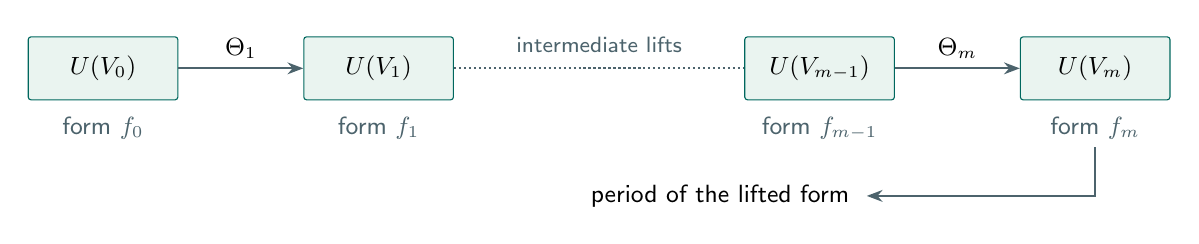
\begin{tikzpicture}[x=1cm,y=1cm]
\foreach \x/\name/\grp in {1/a/0,4.5/b/1,10.1/c/{m-1},13.6/d/m}{
  \node[draw=sea,fill=wash,rounded corners=1pt,minimum width=1.9cm,minimum height=.8cm]
       (\name) at (\x,1.6) {$U(V_{\grp})$};
  \node[below,text=muted] at (\x,1.1) {form $f_{\grp}$};
}
\draw[arrow] (a)--node[above]{$\Theta_1$}(b);
\draw[arrow] (c)--node[above]{$\Theta_m$}(d);
\draw[muted,densely dotted,thick] (b.east)--(c.west);
\node[above,fill=white,font=\sffamily\footnotesize,text=muted] at (7.3,1.68){intermediate lifts};
\draw[arrow] (13.6,.60)--(13.6,-.02)--(10.7,-.02);
\node[anchor=east] at (10.6,-.02){period of the lifted form};
\end{tikzpicture}
\end{document}
